\subsection{②}
  \begin{figure}[H]
    \begin{tabular}{ccc}
      \begin{minipage}{.5\textwidth}
        \centering
        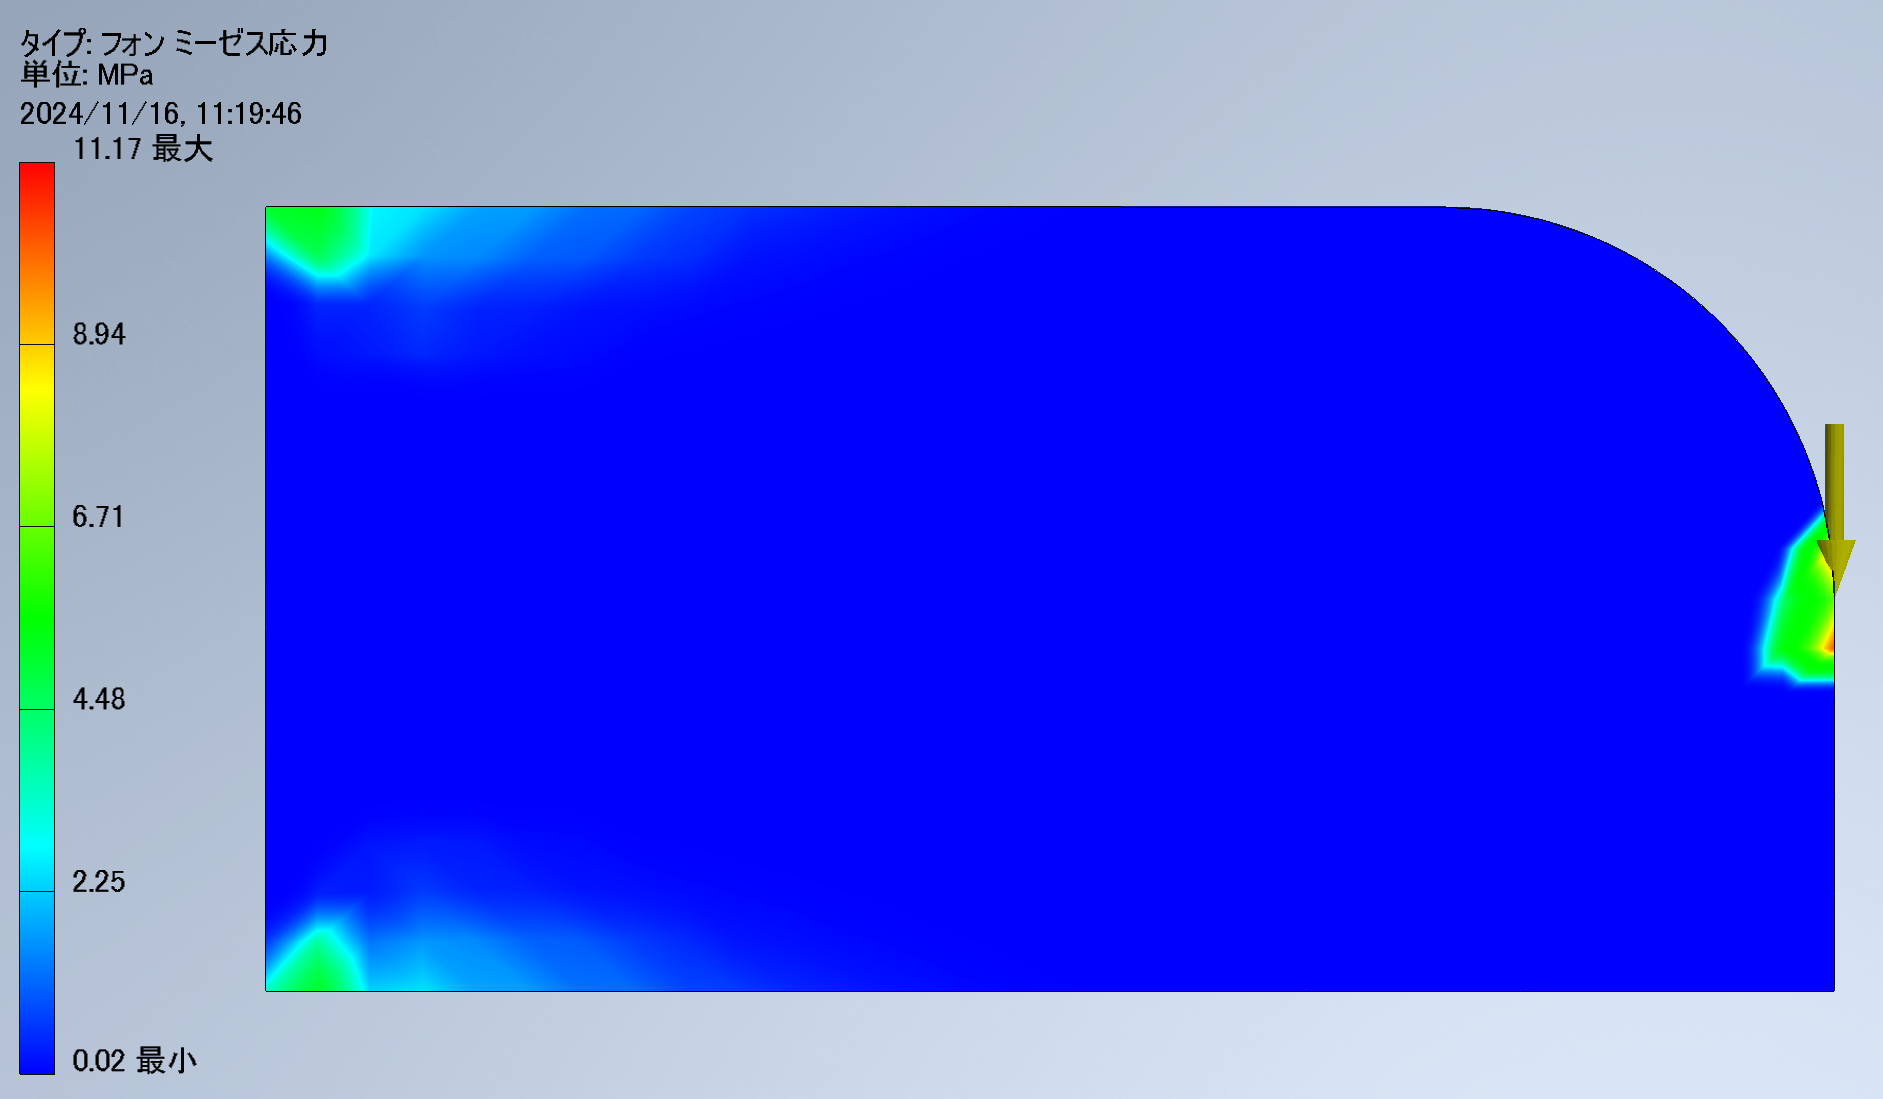
\includegraphics[width=0.99\linewidth]{images/2_voms.png}
        \caption{応力}
        \label{img:2_voms}
      \end{minipage}
      \begin{minipage}{.5\textwidth}
        \centering
        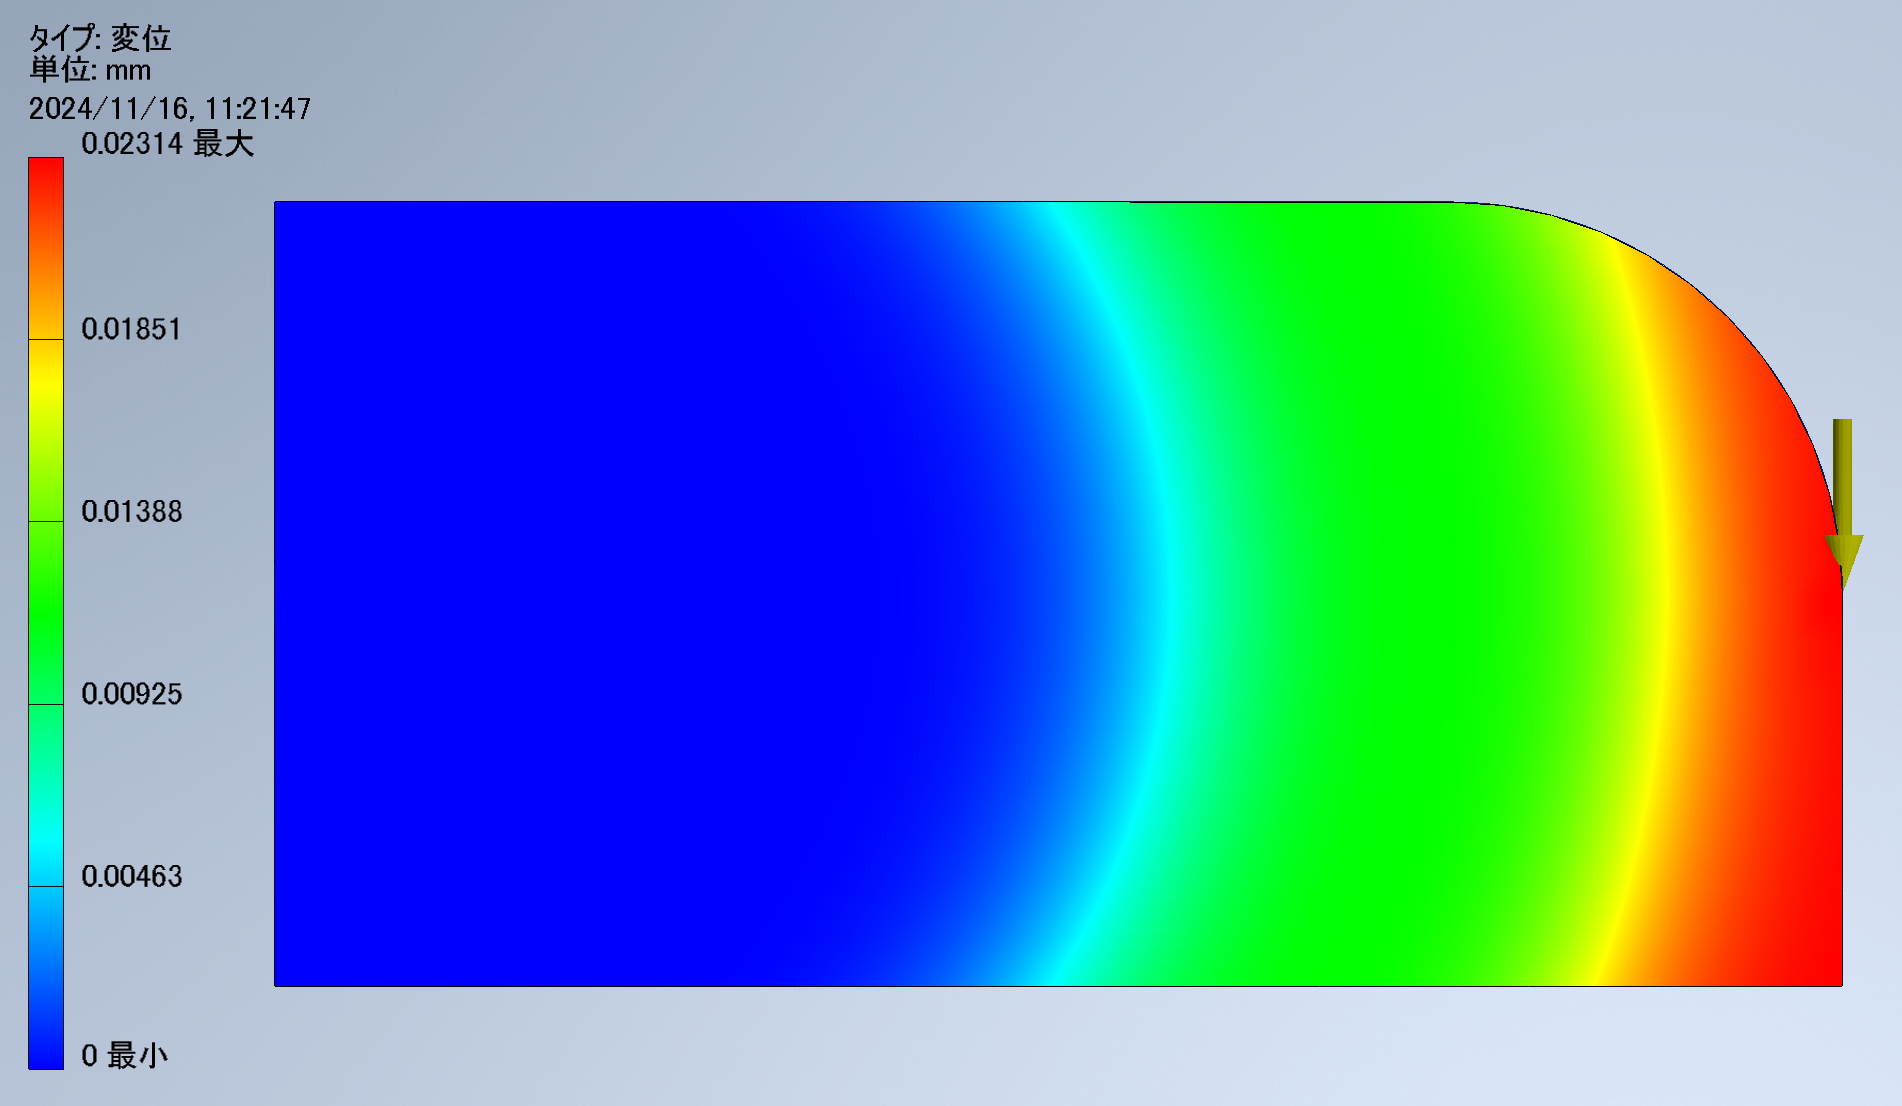
\includegraphics[width=0.99\linewidth]{images/2_disp.png}
        \caption{変位}
        \label{img:2_disp}
      \end{minipage}
    \end{tabular}
  \end{figure}

  以上の図は①で応力が集中してかかっていた辺に,
  半径$48.985[mm]$のフィレットを施して実験を行った結果である.解析条件は以下.
  \begin{equation*}
    V \approx 48430[mm^3]
  \end{equation*}

  図\ref{img:2_voms}からは応力が①よりも分散していることがわかる.
  また応力の最大値が減少はしたが,
  ①より接地面の上下に応力がかかっていることがわかる.
  そして図\ref{img:2_disp}より応力が分散したことにより,
  変位も分散し,最大値が小さくなっていることがわかる.\\\indent
  梁を削って体積が小さくなったのにもかかわらず,
  変位と応力を小さくすることに成功した.\\\indent
  次の実験では右下の辺にもフィレットを施した.
